\documentclass{article}

%Packages
\usepackage[utf8]{inputenc}
\usepackage[margin=1in, letterpaper]{geometry}
\usepackage{amsmath}
\usepackage{amssymb}
\usepackage{graphicx}
\usepackage{wrapfig}
\usepackage{scrextend}
\usepackage{lipsum}
\usepackage{fancyhdr}
\usepackage{subcaption}
\usepackage[usenames,dvipsnames]{xcolor}
\usepackage{tikz}
\usetikzlibrary{calc,trees,positioning,arrows,chains,shapes.geometric,%
	decorations.pathreplacing,decorations.pathmorphing,shapes,%
	matrix,shapes.symbols,plotmarks,decorations.markings,shadows}

%Packages

%Header and Footer
\pagestyle{fancy}
\fancyhead{}
\fancyhead[R]{HW 1}
\fancyhead[L]{Mark Mekosh}
\fancyhead[C]{Computational Physics}
\fancyfoot[C]{\thepage}
%Header and Footer

%\graphicspath{{./images/}}
\definecolor{lec1}{RGB}{120,170,230}
\definecolor{lec2}{RGB}{220,220,220}

%Commands
\newcommand{\hrt}{\begin{center} \line(1,0){469} \line(0,-1){15} \end{center}}
\newcommand{\hrb}{\begin{center} \line(1,0){469} \line(0,1){15} \end{center}}
\newcommand{\cbox}[2]{\begin{center} \fbox{\begin{minipage}{#1em} \begin{center}#2\end{center} \end{minipage}} \end{center}}
\newcommand{\titledbox}[3]{}
\newcommand{\dv}[1]{\dot{\vec{#1}}}
\newcommand{\ddv}[1]{\ddot{\vec{#1}}}
\newcommand{\cross}[2]{#1 \times #2}
\newcommand{\Lagr}{\mathcal{L}}
\newcommand{\code}[1]{\begin{addmargin}[2em]{2em} \textcolor{blue} {\fontfamily{pcr}\selectfont #1} \end{addmargin}}
\newcommand{\codeout}[1]{\begin{addmargin}[2em]{2em} \textbf{Output:} \\ \color{Green} {\fontfamily{qcr}\selectfont #1} \end{addmargin}}
\newcommand{\ex}[3]{\hrt \subsection*{Exercise #1} \textbf{\underline{Q:}} \\ #2 \\ \textbf{\underline{A:}} \\ #3 \hrb}
\newcommand{\eq}[3]{\hrt \subsection*{Example #1} \textbf{\underline{Q:}} \\ #2 \\ \textbf{\underline{A:}} \\ #3 \hrb}
\newcommand{\imageleft}[2]{\begin{wrapfigure}{l}{#1\textwidth} \includegraphics[width=#1\textwidth]{#2} \end{wrapfigure}}
\newcommand{\imageright}[2]{\begin{wrapfigure}{r}{#1\textwidth} \includegraphics[width=#1\textwidth]{#2} \end{wrapfigure}}
\newcommand{\homework}[3]{\flushleft Mark Mekosh \\ #1 \\ #2 \\ #3}
\newcommand{\deriv}[2]{\frac{d #1}{d #2}}
\newcommand{\pderiv}[2]{\frac{\partial #1}{\partial #2}}
\newcommand{\dprod}[2]{\vec{#1} \cdot \vec{#2}}

%Commands


\begin{document}
\homework{1/28/20}{Phys 510}{Homework $\#1$}

\section*{1}

	\subsection*{a)}
		-1/3 $\approx$ -0.33333334 $=$ 10111110101010101010101010101011
	\subsection*{b)}
		\begin{gather}
			x_1 = 0.11258762\times 10^2 \ \ \& \ \  x_2 = 0.11244891 \times 10^2 \\
			x_1 + x_2 = (0.11258762 \times 10^2) + (0.11244891 \times 10^2) \\
			= ( 0.11258762 + 0.11244891) \times 10^2 \\
			= ( 0.22503653) \times 10^2 \\
			= 22.50
			\intertext{relative error = $(22.503653 - 22.50)/22.503653 = 0.0162\%$}
			x_1 - x_2 = ( 0.11258762 \times 10^2 ) + (0.11244891 \times 10^2) \\
			= (0.11258762 - 0.11244891) \times 10^2 \\
			= (0.00013871000000000022) \times 10^2 \\
			= (0.0001 \times 10^2)
			= 0.01 \\
			\intertext{relative error = $(0.0139 - 0.01)/0.0139 = 28.06\%$}
		\end{gather}
	\subsection*{c)}
		16777217
	\subsection*{d)}
		\begin{gather}
			\exp(x) = \sum_{k=0}^{\infty} \frac{x^k}{k!}
			\intertext{For single precision we have $e^1 = 2.7182817$ and for double precision we have $e^1 = 2.718281828459045$}
			\intertext{For k summed up to 10 and beyond we have $e^1 = 2.7182817$}
			\intertext{For k summed up to 17 and beyond we have $e^1 = 2.718281828459045$}
		\end{gather}
	\subsection*{e)}
		Machine epsilon for single precision $2^{-23} = 1.1920929 \times 10^{-7}$ \\
		Machine epsilon for double precision $2^{-52} = 2.220446049250313 \times 10^{-16}$
		
\section*{3}
	\begin{figure}[h]
		\begin{subfigure}{0.5\textwidth}
			\centering
			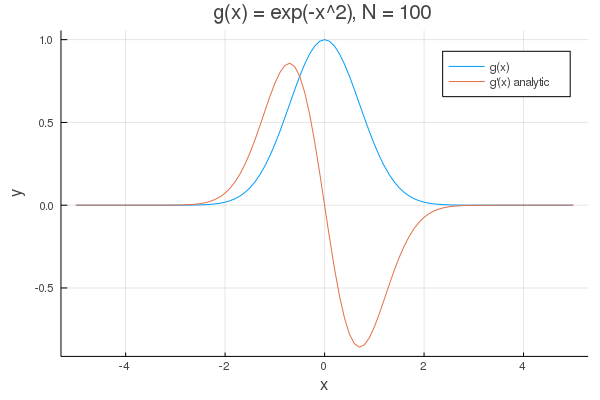
\includegraphics[scale=0.4]{"C:/users/markm/documents/grad school/year 1.5/phys510/homework/homework1/g_plot.png"}
		\end{subfigure}
		\begin{subfigure}{0.5\textwidth}
			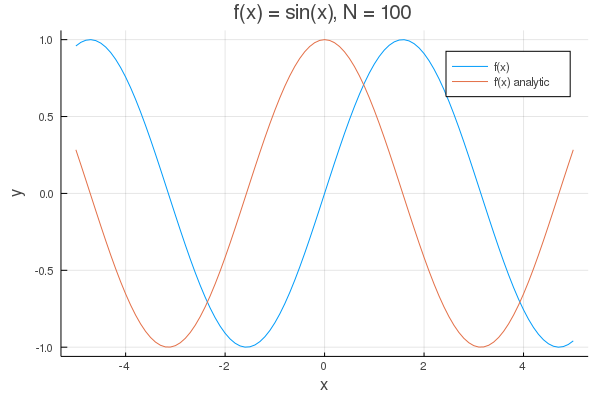
\includegraphics[scale=0.4]{"C:/users/markm/documents/grad school/year 1.5/phys510/homework/homework1/f_plot.png"}
		\end{subfigure}
	\end{figure}

		\begin{figure}[h]
		\begin{subfigure}{0.5\textwidth}
			\centering
			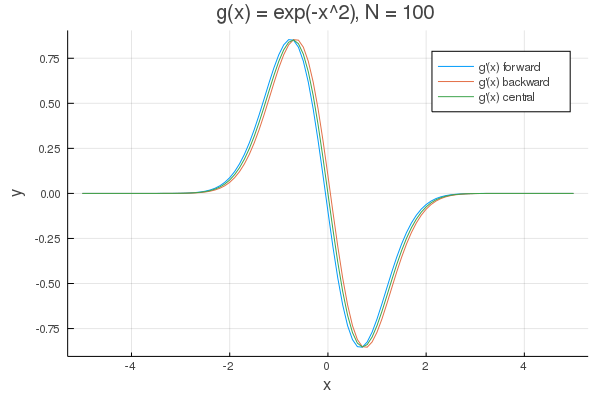
\includegraphics[scale=0.4]{"C:/users/markm/documents/grad school/year 1.5/phys510/homework/homework1/g_plot2.png"}
		\end{subfigure}
		\begin{subfigure}{0.5\textwidth}
			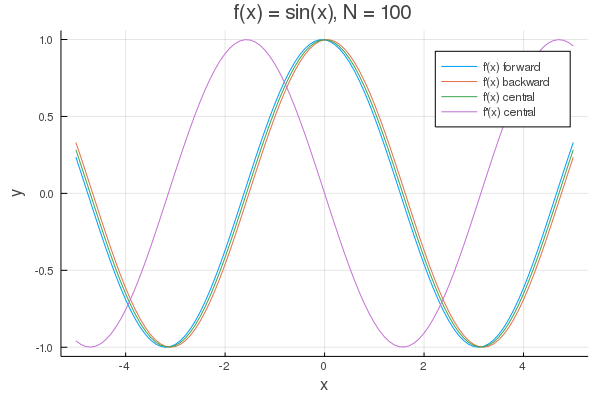
\includegraphics[scale=0.4]{"C:/users/markm/documents/grad school/year 1.5/phys510/homework/homework1/f_plot2.png"}
		\end{subfigure}
	\end{figure}

\end{document}